\begin{tikzpicture}
\node[anchor=south west,inner sep=0] at (0,0) {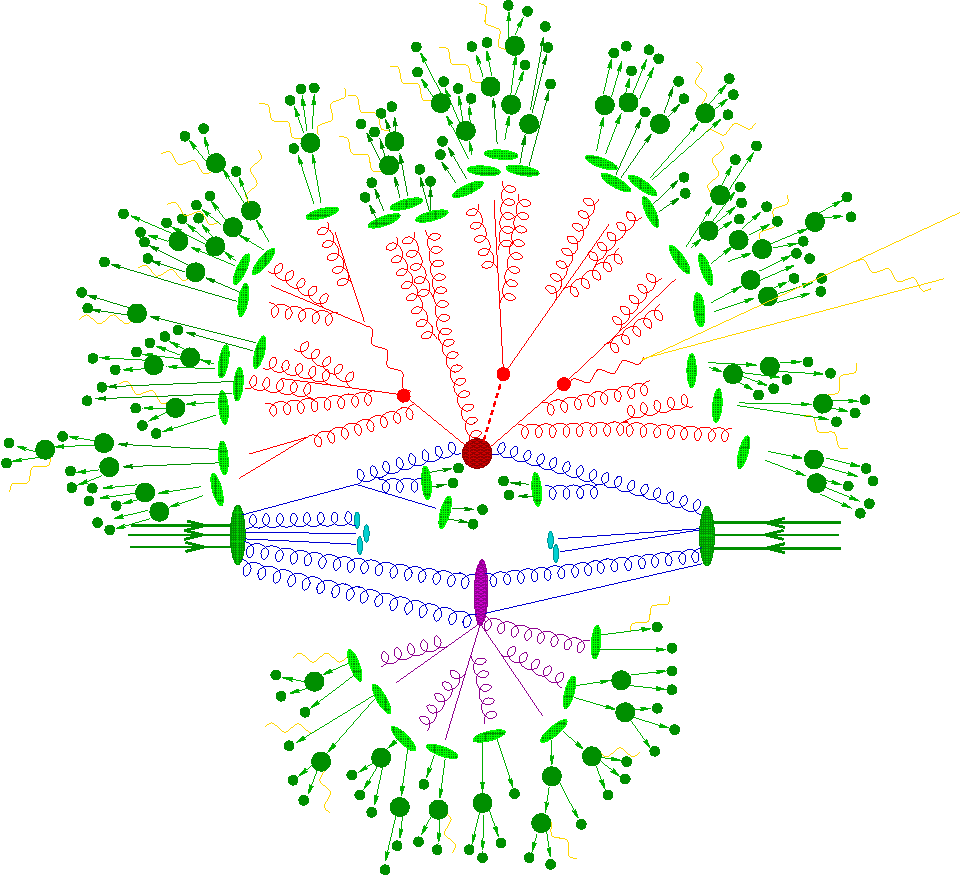
\includegraphics[width=15cm]{\PhDthesisdir/plots_and_images/from_event_generator_HEP/2-Figure1-1.png}};

\draw [thick, latex-] (3.6, 4.8) --+ (-155:1.5) node [left] {proton};
\draw [thick, latex-] (11.2, 4.8) --+ (-25:1.5) node [right] {proton};

\draw [thick, decorate, decoration={brace, amplitude=5pt}] (10.8,4.5)  -- (10.8,0);
\draw (11,2.25) node [right] {Événement sous-jacent};

\draw (7.5, 7.2) node {Événement dur};
\draw (7.5, 8.5) node {Gerbe partonique};
\draw (5, 13) node {Hadronisation};

\end{tikzpicture}
